\subsection{Introduction}
Recall a question we had on the worksheet last week:
\begin{center}
\textit{``Draw the locus of points that are exactly 3 cm away from a point A''}
\end{center}

Maybe you tried it...maybe you didn't. But hopefully now that you've done it, you realize that I was asking you to draw a circle all along! So what is so mystical about the circle? The ancients seemed to fawn over its perfection and worship its impeccable symmetry. What we will find out is that there are many interesting geometric properties about circles.

\subsection{Basics}
\begin{center}
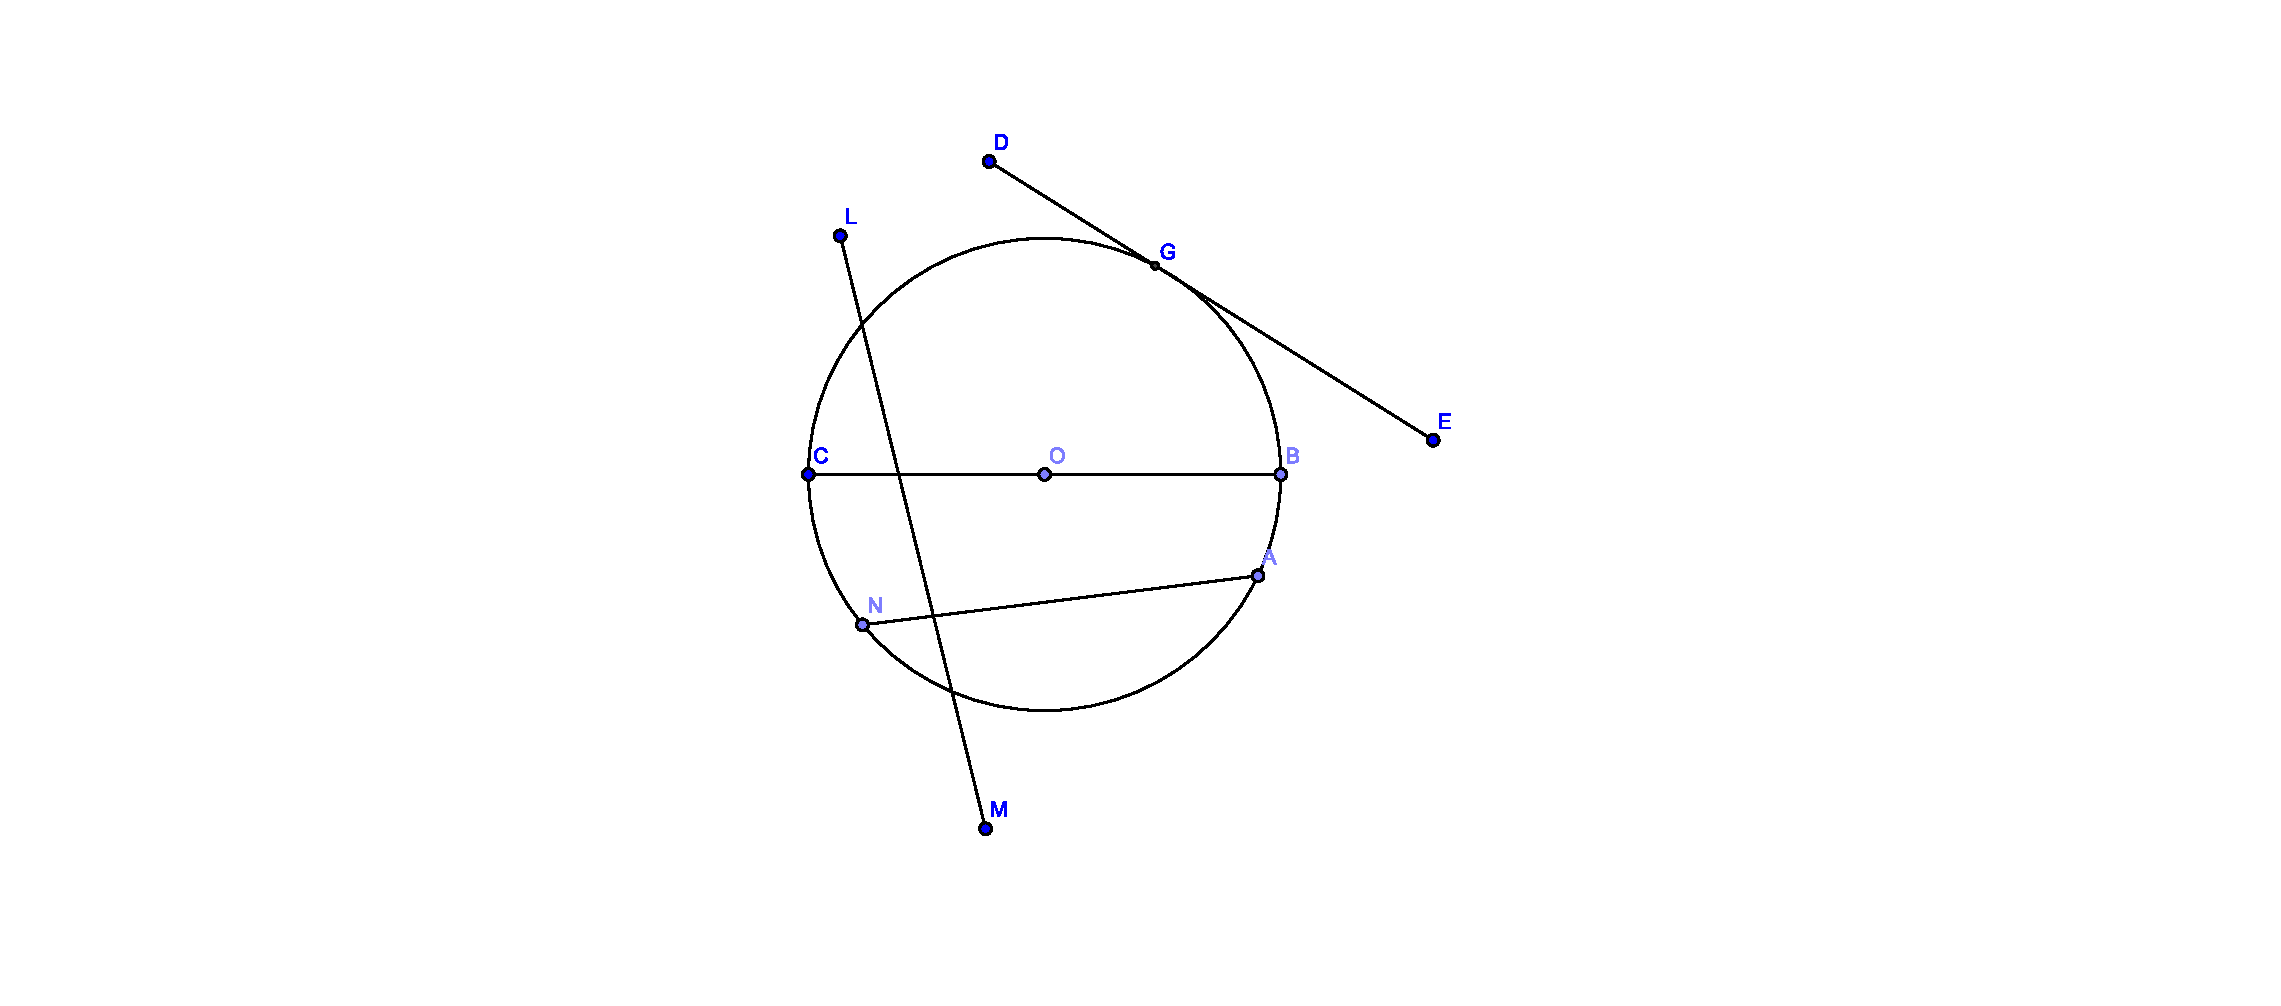
\includegraphics[height=3in, trim={2cm 1cm 0 1.1cm}]{circle1}
\end{center}
We start off with a circle, which as we see from our definition earlier, is a collection of points that are equidistant from a particular point. In general, we often use \textbf{O} as the center of the circle (origin). Now, on this circle we can draw many special lines:
\begin{itemize}
    \item The \textbf{radius} is the line from the center to any point on the circle On the diagram, $\overline{OC}$ and $\overline{OB}$ are both radii. 
    \item The \textbf{diameter} is defined to be the line through the center of the circle. Note that the length of the diameter is $2r$, where $r$ is the radius of the circle.
    \item A \textbf{chord} is any line connecting any two non-equal points on the circle. Note that the diameter is a special case of a chord
    \item A \textbf{secant} is any line intersecting the circle at two points
    \item A \textbf{tangent} is any line intersecting the circle at exactly one point
\end{itemize}

\subsubsection{$\pi$}
In order to prove some basic theorems, we have to begin with this theorem,

\begin{theorem}
The ratio of the circumference of a circle to its diameter is $\pi$
\end{theorem}

Or in equation form, $\text{Circumference} = \pi d = 2\pi r$. As you guys probably already know, $\pi = 3.14159\cdots$. With this knowledge, we can prove the area of a circle.

\begin{theorem}
The area of a circle is $\pi r^2$
\end{theorem}

\subsection{Angles}
Now that we know what a circle is, it is natural to begin a discussion of how angles are related to a circle. 
\begin{center}
\begin{tikzpicture}
% the origin
\coordinate (O) at (0,0);
% the circle and the dot at the origin
\draw (O) node[circle,inner sep=1.5pt,fill] {} circle [radius=3cm];
\draw (O) node[left] {$O$};
\draw (3cm,0) node[right] {$A$};
\draw (60:3cm) node[right, above] {$B$};
% the ``\theta'' arc
\draw 
  (3cm,0) coordinate (xcoord) -- 
  node[midway,below] {$r$} (O) -- 
  (60:3cm) coordinate (slcoord)
  pic [draw,->,angle radius=1cm,"$\theta$"] {angle = xcoord--O--slcoord};

\end{tikzpicture}
\end{center}

We define an \textbf{angle} to be the figure formed by two \textbf{rays}. If we consider the diagram above, the angle has \textbf{measure} $\theta$ and \textbf{subtends} $\arc{AB}$. We usually refer to an angle to either the vertex it is at, or to avoid confusion, the acute angle formed by three points---in our case, $\angle ABO$ or $\angle BOA$.

As you may know, a circle contains $360\degree$. It turns out, this number was entirely arbitrary, as in we could've chosen 100 or 1000. But we have 360, because it's divisible by a bunch of numbers, and that's what we still use today. There is also another way to define angles, called \textbf{radians}. The conversion for this is 
$$1 = \frac{360\degree}{2\pi}.$$
Until you are in higher math or physics, you won't be needing radians too much.

When we have an angle, we can classify it into three categories, 
\begin{itemize}
    \item \textbf{Acute}: $<90\degree$
    \item \textbf{Right, Perpendicular, Orthogonal}: $=90\degree$
    \item \textbf{Obtuse}: $>90\degree$
    \item \textbf{Reflex}: $>180\degree$
\end{itemize}
We also say two angles whose sum is $90\degree$ are \textbf{complementary}, and two angles whose sum is $180\degree$ is \textbf{supplementary}. If you ever get confused, just remember that ``a compliment is the \textit{right} thing to do!'' Note that this compliment is spelled differently, but nonetheless still is useful for memorizing the term. 
\newpage
\subsubsection{Lines in a Circle}
From our diagram above, it is clear that the angle formed by the rays equals the arc of the circle. This type of angle is known as a \textbf{central angle}, and is the easiest to deal with. For the other angles, they have certain formulas. We will look at them and try to prove their properties as well. \vspace{0.2in}

\begin{minipage}{0.6\textwidth}
\subsubsection{Inscribed Angle}
\begin{center}
\begin{tikzpicture}
\draw (0,0) circle  [radius = 3cm];
\draw (-30:3cm) coordinate (a) node[right] {$A$}  --
 (200:3cm) coordinate (b) node[left] {$B$}  --
(60:3cm) coordinate (c) node[right, above] {$C$} ;
\pic [draw,-,angle radius=1cm,"$\theta$"] {angle = a--b--c};
\end{tikzpicture}
\end{center}
\end{minipage}
\begin{minipage}{0.35\textwidth}
$$\theta = \frac{\arc{AC}}{2}.$$
\end{minipage}

\vspace{1in}

\subsubsection{Two Secants}
\begin{minipage}{0.6\textwidth}
\begin{center}
\begin{tikzpicture}
\draw (0,0) circle  [radius = 3cm];
\draw (15:3cm) node[right] {$\alpha$};
\draw (190:3cm) node[right] {$\beta$};
\draw (-30:3cm) coordinate (a) node[right] {$A$}  --
 (-5cm, -1cm) coordinate (b) node[left] {$B$}  --
(60:3cm) coordinate (c) node[right, above] {$C$} ;
\pic [draw,-,angle radius=1cm,"$\theta$"] {angle = a--b--c};
\end{tikzpicture}
\end{center}
\end{minipage}
\begin{minipage}{0.35\textwidth}
$$\theta = \frac{\alpha-\beta}{2} $$
Note that there is a similar formula for two tangents.
\end{minipage}

\subsubsection{Tangent and Chord}
\begin{minipage}{0.6\textwidth}
\begin{center}
\begin{tikzpicture}
\draw (0,0) circle  [radius = 3cm];
\draw (3,-3) coordinate (a) node[right] {$A$}--
(-3,-3) coordinate (b) node[left] {$B$};
\draw (0,-3) coordinate (o) node[below] {$D$}--
(60:3cm) coordinate (c) node[right, above] {$C$} ;
\pic [draw,-,angle radius=1cm,"$\theta$"] {angle = a--o--c};
\end{tikzpicture}
\end{center}
\end{minipage}
\begin{minipage}{0.35\textwidth}
This is actually just a special case of the theorem above.
$$\theta = \frac{\arc{DC}}{2}$$
\end{minipage}

\vspace{1in}

\subsubsection{Two Chords}
\begin{minipage}{0.6\textwidth}
\begin{center}
\begin{tikzpicture}
\draw (0,0) circle  [radius = 3cm];
\draw (165:3cm) node[left] {$\alpha$};
\draw (5:3cm) node[right] {$\beta$};
\draw[name path = a--b] (200:3cm) coordinate (a) node[left] {$A$}  --
 (30:3cm) coordinate (b) node[right] {$B$};
 \draw[name path = c--d] (-20:3cm) coordinate (c) node[right] {$C$}  --
 (130:3cm) coordinate (d) node[left] {$D$};
\path [name intersections={of=a--b and c--d,by=o}];
\node [fill=black,inner sep=1pt,label=-90:$O$] at (o) {};
\pic [draw,-,angle radius=1cm,"$\theta$"] {angle = c--o--b};
\end{tikzpicture}
\end{center}
\end{minipage}
\begin{minipage}{0.35\textwidth}
$$\theta = \frac{\alpha+\beta}{2}$$
\end{minipage}

\subsection{Problems}
\begin{problem}
Prove that the angle formed by the intersection of a tangent and a radius of a circle is $90\degree$.
\end{problem}
\begin{problem}
Show that any triangle inscribed in a circle with the diameter as one of its sides must be a right triangle.
\end{problem}
\begin{problem}
Show that the length of the segment connecting the $90\degree$ vertex of a right triangle to the midpoint of the hypotenuse is equal to half the hypotenuse.
\end{problem}
\begin{problem}
Prove that the angles of a triangle must sum to $180\degree$.
\end{problem}

\clearpage
\begin{problem}
(MATHCOUNTS State Sprint \#30 2009) In the figure, the measure of angle RAS is 74 degrees, and the measure of angle RTB is 28 degrees. What is the measure of minor arc BR, in degrees?
\begin{center}
\includegraphics[height=2in]{circleMath}
\end{center}
\end{problem}
\vspace{1.5in}
\section{Power of a Point}
As you can imagine, these theorems are very powerful. But in all seriousness, now that we've done angles, it's time to learn about how side lengths are related in circles.

\subsubsection{Equal Tangents}
\begin{minipage}{0.6\textwidth}
\begin{center}
\begin{tikzpicture}
\draw (0,0) circle  [radius = 3cm];
\draw (111:3cm) coordinate (a) node[above] {$B$}  --
 (-6cm, 0.3cm) coordinate (b) node[left] {$A$}  --
(235:3cm) coordinate (c) node[below ] {$C$} ;
\end{tikzpicture}
\end{center}
\end{minipage}
\begin{minipage}{0.35\textwidth}
\begin{theorem}
Two tangents from the same point to a circle are always equal.
\end{theorem}
In other words, $AB = AC$.
\end{minipage}

\subsubsection{General Case}
\begin{minipage}{0.6\textwidth}
\begin{center}
\begin{tikzpicture}
\draw (0,0) circle  [radius = 3cm];
\draw (141:3cm) node[left] {$B$};
\draw (-162:3cm) node[left] {$D$};
\draw (80:3cm) coordinate (a) node[above] {$C$}  --
 (-6cm, 0.3cm) coordinate (b) node[left] {$A$}  --
(-50:3cm) coordinate (c) node[below ] {$E$} ;
\end{tikzpicture}
\end{center}
\end{minipage}
\begin{minipage}{0.35\textwidth}
$$(\overline{AB})(\overline{AC})=(\overline{AD})(\overline{AE})$$
\end{minipage}

\subsubsection{Special Case}
\begin{minipage}{0.6\textwidth}
\begin{center}
\begin{tikzpicture}
\draw (0,0) circle  [radius = 3cm];
\draw (205:3cm) node[left] {$C$};
\draw (111:3cm) coordinate (a) node[above] {$B$}  --
 (-6cm, 0.3cm) coordinate (b) node[left] {$A$}  --
(-70:3cm) coordinate (c) node[below ] {$D$} ;
\end{tikzpicture}
\end{center}
\end{minipage}
\begin{minipage}{0.35\textwidth}
A special case of the theorem above.
$$(\overline{AC})(\overline{AD}) = \overline{AB}^2$$
\end{minipage}

\subsubsection{Two Chords}
\begin{minipage}{0.6\textwidth}
\begin{center}
\begin{tikzpicture}
\draw (0,0) circle  [radius = 3cm];
\draw[name path = a--b] (200:3cm) coordinate (a) node[left] {$A$}  --
 (30:3cm) coordinate (b) node[right] {$B$};
 \draw[name path = c--d] (-20:3cm) coordinate (c) node[right] {$C$}  --
 (130:3cm) coordinate (d) node[left] {$D$};
\path [name intersections={of=a--b and c--d,by=o}];
\node [fill=black,inner sep=1pt,label=-90:$O$] at (o) {};
\end{tikzpicture}
\end{center}
\end{minipage}
\begin{minipage}{0.35\textwidth}
$$(\overline{OA})(\overline{OB})=(\overline{OD})(\overline{OC})$$
\end{minipage}

\subsection{Problems}
\begin{problem}
Prove that if a circle can be inscribed in quadrilateral $ABCD$, then $AB+CD=BC+AD$.
\end{problem}
\begin{problem}
Express all the line segments of a triangle purely in terms of its side lengths when its incircle is drawn.
\end{problem}
\begin{problem}
Prove that if a radius bisects a chord, then it is perpendicular to the chord.
\end{problem}
\begin{problem}
Prove that if a radius intersects a chord perpendicularly, then it must bisect the chord.
\end{problem}
\begin{problem}
(AHSME 1954) A point $P$ is outside a circle and is $13$ inches from the center. A secant from $P$ cuts the circle at $Q$ and $R$ so that the external segment of the secant $PQ$ is $9$ inches and $QR$ is $7$ inches. The radius of the circle is:

$\textbf{(A)}\ 3" \qquad \textbf{(B)}\ 4" \qquad \textbf{(C)}\ 5" \qquad \textbf{(D)}\ 6"\qquad\textbf{(E)}\ 7"$
\end{problem}
\begin{problem}
(AHSME 1956) The points $A$, $B$, and $C$ are on circle $O$. THe tangent line at $A$ and the secant $BC$ intersect at $P$, $B$, lying between $C$ and $P$. If $BC=20$ and $PA=10\sqrt{3}$, find $PB$.
\end{problem}
\begin{problem}
The figure below, $O$ is the center of circle $O$, $\overline{AD}=6$, $\overline{OD}=9$, and $\overline{AB} = 2\overline{BC}$. Find $\overline{AB}$.
\begin{center}
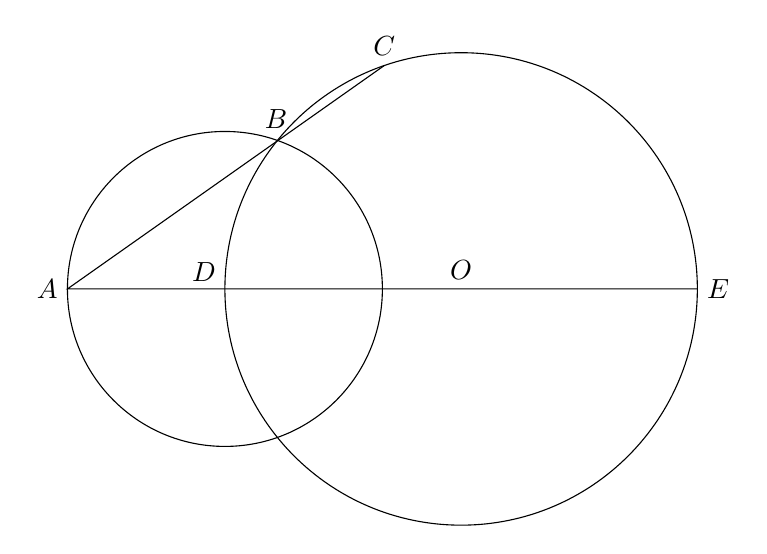
\begin{tikzpicture}
\draw (0,0) circle  [radius = 3cm];
\draw (0,0) node[above] {$O$};
\draw (-3,0) circle [radius = 2.0cm]; 
\draw (134:3cm) node[left] {$B$};
\draw (176:3cm) node[left] {$D$};
\draw (109:3cm) coordinate (a) node[above] {$C$}  --
 (-5.0cm, 0) coordinate (b) node[left] {$A$}  --
(0:3cm) coordinate (c) node[right] {$E$} ;
\end{tikzpicture}
\end{center}
\end{problem}
\begin{problem}
Two tangents from an external point $P$ are drawn to a circle and intersect it at $A$ and $B$. A third tangent meets the circle at $T$, and the tangents $\overline{PA}$ and $\overline{PB}$ at points $Q$ and $R$, respectively. If $AB=20$, then find the perimeter of $\triangle PQR$.
\end{problem}